\documentclass[a4paper,onecolumn,oneside,12pt,extrafontsizes]{memoir}
\pdfinclusioncopyfonts 1

%\usepackage[cp1250]{inputenc}

\usepackage[polish]{babel}
\usepackage{ebgaramond} 
\usepackage[utf8]{inputenc}
\usepackage[T1]{fontenc}
\usepackage{tgtermes} 
\frenchspacing


\usepackage{setspace}

\usepackage{tabularx}

\usepackage{color,calc}

\renewcommand*\ttdefault{txtt}

\usepackage{listings} 		% pakiet do prezentacji kodu.
\usepackage{MnSymbol} 
\lstdefinestyle{customcpp} {
	belowcaptionskip=1\baselineskip,
	language=C++,
	basicstyle=\footnotesize\ttfamily,
	frame=single,
	showstringspaces=false,
	tabsize=4,
	breaklines=true,
	breakatwhitespace=true,
	prebreak={ \space },
	postbreak=\raisebox{0ex}[0ex][0ex]{\ensuremath{\rcurvearrowse\space}},
	escapeinside={@}{@}
}
\lstset{style=customcpp}

%\usepackage{minted}

\clubpenalty=10000			%kara za sierotki
\widowpenalty=10000			% nie pozostawiaj wdów
\brokenpenalty=10000		% nie dziel wyrazów między stronami
\exhyphenpenalty=999999		% nie dziel słów z myślnikiem
\righthyphenmin=3			% dziel minimum 3 litery

%\usepackage{polski}
%\usepackage[draft,nosingleletter]{impnattypo}

\renewcommand{\topfraction}{0.95}
\renewcommand{\bottomfraction}{0.95}
\renewcommand{\textfraction}{0.05}
\renewcommand{\floatpagefraction}{0.35}

\usepackage{todonotes}

%%%%%%%%%%%%%%%%%%%%%%%%%%%%%%%%%%%%%%%%%%%%%%%%%%%

%%  Ustawienia rozmiarów: tekstu, nagłówka i stopki, marginesów

%%  dla dokumentów klasy memoir

%%%%%%%%%%%%%%%%%%%%%%%%%%%%%%%%%%%%%%%%%%%%%%%%%%%

\setlength{\headsep}{10pt}
\setlength{\headheight}{13.6pt} % wartość baselineskip dla czcionki 11pt tj. \small wynosi 13.6pt
\setlength{\footskip}{\headsep+\headheight}
\setlength{\uppermargin}{\headheight+\headsep+1cm}
\setlength{\textheight}{\paperheight-\uppermargin-\footskip-1.5cm}
\setlength{\textwidth}{\paperwidth-5cm}
\setlength{\spinemargin}{2.5cm}
\setlength{\foremargin}{2.5cm}
\setlength{\marginparsep}{2mm}
\setlength{\marginparwidth}{2.3mm}
\checkandfixthelayout[fixed] % konieczne, aby się dobrze wszystko poustawiało

%%%%%%%%%%%%%%%%%%%%%%%%%%%%%%%%%%%%%%%%%%%%%%%%

%%  Ustawienia odległości linii, wcięć, odstępów

%%%%%%%%%%%%%%%%%%%%%%%%%%%%%%%%%%%%%%%%%%%%%%%%

\linespread{1}
\setlength{\parindent}{14.5pt}

%%%%%%%%%%%%%%%%%%%%%%%%%%%%%%%%%%%%%%%%%%%%%%%%%%%

%%  Pakiety i komendy zastosowane tylko do zamieszczenia informacji o użytych komendach i fontach

%%  Normalnie nie są potrzebne, można je zamarkować podczas redakcji pracy

%%%%%%%%%%%%%%%%%%%%%%%%%%%%%%%%%%%%%%%%%%%%%%%%%%%

%\usepackage{memlays}     % extra layout diagrams, zastosowane w szblonie do 'debuggowania', używa pakietu layouts
\usepackage{printlen} % pakiet do wyświetlania wartości zdefiniowanych długości, stosowany do 'debuggowania'
\uselengthunit{pt}
\makeatletter
\newcommand{\showFontSize}{\f@size pt} % makro wypisujące wielkość bieżącej czcionki
\makeatother

% do pokazania ramek można byłoby użyć:
%\usepackage{showframe}

%%%%%%%%%%%%%%%%%%%%%%%%%%%%%%%%%%%%%%%%%%%%%%%%%%%

%%  Formatowanie list wyliczeniowych, wypunktowań i własnych otoczeń

%%%%%%%%%%%%%%%%%%%%%%%%%%%%%%%%%%%%%%%%%%%%%%%%%%%


\usepackage{enumitem} % pakiet pozwalający zarządzać formatowaniem list wyliczeniowych
\setlist{noitemsep,topsep=4pt,parsep=0pt,partopsep=4pt,leftmargin=*} % zadeklarowane parametry pozwalają uzyskać 'zwartą' postać wypunktowania bądź wyliczenia
\setenumerate{labelindent=0pt,itemindent=0pt,leftmargin=!,label=\arabic*.} % można zmienić \arabic na \alph, jeśli wyliczenia mają być z literkami
\setlistdepth{4} % definiujemy głębokość zagnieżdżenia list wyliczeniowych do 4 poziomów
\setlist[itemize,1]{label=$\bullet$}  % definiujemy, jaki symbol ma być użyty w wyliczeniu na danym poziomie
\setlist[itemize,2]{label=\normalfont\bfseries\textendash}
\setlist[itemize,3]{label=$\ast$}
\setlist[itemize,4]{label=$\cdot$}
\renewlist{itemize}{itemize}{4}

\makeatletter
\renewenvironment{quote}{
\begin{list}{}
{
\setlength{\leftmargin}{1em}
\setlength{\topsep}{0pt}%
\setlength{\partopsep}{0pt}%
\setlength{\parskip}{0pt}%
\setlength{\parsep}{0pt}%
\setlength{\itemsep}{0pt}
}
}{
\end{list}}
\makeatother

%%%%%%%%%%%%%%%%%%%%%%%%%%%%%%%%%%%%%%%%%

%%  Pakiet do generowania indeksu (ważne, aby wstawić przed hyperref)

%%%%%%%%%%%%%%%%%%%%%%%%%%%%%%%%%%%%%%%%%

\DisemulatePackage{imakeidx}
\usepackage[makeindex,noautomatic]{imakeidx} % tutaj mówimy, żeby indeks nie generował się automatycznie,
\makeindex
\makeatletter
\makeatother


\usepackage{ifpdf}
\ifpdf
	\usepackage[pdftex,bookmarks,breaklinks,unicode]{hyperref}
	%\usepackage[pdftex]{graphicx}
	\DeclareGraphicsExtensions{.pdf,.jpg,.mps,.png}
\pdfcompresslevel=9
\pdfoutput=1
\makeatletter
\AtBeginDocument{
	\hypersetup{
		pdfinfo={
		Title = {\@title},
		Author = {\@author},
		Subject={},
		Keywords={słowa kluczowe},
		}}
}
\makeatother
\else
\usepackage{graphicx}
\DeclareGraphicsExtensions{.eps,.ps,.jpg,.mps,.png}
\fi
\sloppy

% Deklaracja głębokościu numeracji
\setcounter{secnumdepth}{2}
\setcounter{tocdepth}{2}
\setsecnumdepth{subsection} % activating subsubsec numbering in doc

% Kropki po numerach sekcji
\makeatletter
\def\@seccntformat#1{\csname the#1\endcsname.\quad}
\def\numberline#1{\hb@xt@\@tempdima{#1\if&#1&\else.\fi\hfil}}
\makeatother

\renewcommand{\chapternumberline}[1]{#1.\quad}
\renewcommand{\cftchapterdotsep}{\cftdotsep}

% Czcionka do podpisów tabel i rysunków
\captionnamefont{\small}
\captiontitlefont{\small}

% Przedefiniowanie etykiet w podpisach tabel i rysunków
%\AtBeginDocument{%
    \addto\captionspolish{%
    \renewcommand{\tablename}{Tab.}%
}%}

%\AtBeginDocument{%
    \addto\captionspolish{%
    \renewcommand{\figurename}{Rys.}%
}%}

%\AtBeginDocument{%
    \addto\captionspolish{%
    \renewcommand{\bibname}{Literatura}%
}%}

%\AtBeginDocument{%
    \addto\captionspolish{%
    \renewcommand{\listfigurename}{Spis rysunków}%
}%}

%\AtBeginDocument{%
    \addto\captionspolish{%
    \renewcommand{\listtablename}{Spis tabel}%
}%}

%\AtBeginDocument{%
    \addto\captionspolish

%%%%%%%%%%%%%%%%%%%%%%%%%%%%%%%%%%%%%%%%%%%%%%%%%%%%%%%%%%%%%%%%%%

%% Definicje stopek i nagłówków

%%%%%%%%%%%%%%%%%%%%%%%%%%%%%%%%%%%%%%%%%%%%%%%%%%%%%%%%%%%%%%%%%%

\addtopsmarks{headings}{%
\nouppercaseheads % added at the beginning
}{%

\createmark{chapter}{both}{shownumber}{}{. \space}
%\createmark{chapter}{left}{shownumber}{}{. \space}
\createmark{section}{right}{shownumber}{}{. \space}
}%use the new settings

\makeatletter
\copypagestyle{outer}{headings}
\makeoddhead{outer}{}{}{\small\itshape\rightmark}
\makeevenhead{outer}{\small\itshape\leftmark}{}{}
\makeoddfoot{outer}{\small\@author:~\@titleShort}{}{\small\thepage}
\makeevenfoot{outer}{\small\thepage}{}{\small\@author:~\@title}
\makeheadrule{outer}{\linewidth}{\normalrulethickness}
\makefootrule{outer}{\linewidth}{\normalrulethickness}{2pt}
\makeatother

% fix plain
\copypagestyle{plain}{headings} % overwrite plain with outer
\makeoddhead{plain}{}{}{} % remove right header
\makeevenhead{plain}{}{}{} % remove left header
\makeevenfoot{plain}{}{}{}
\makeoddfoot{plain}{}{}{}

\copypagestyle{empty}{headings} % overwrite plain with outer
\makeoddhead{empty}{}{}{} % remove right header
\makeevenhead{empty}{}{}{} % remove left header
\makeevenfoot{empty}{}{}{}
\makeoddfoot{empty}{}{}{}



%%%%%%%%%%%%%%%%%%%%%%%%%%%%%%%%%%%%%%%

%% Definicja strony tytułowej

%%%%%%%%%%%%%%%%%%%%%%%%%%%%%%%%%%%%%%%
\makeatletter
%Uczelnia
\newcommand\uczelnia[1]{\renewcommand\@uczelnia{#1}}
\newcommand\@uczelnia{}

%Wydział
\newcommand\wydzial[1]{\renewcommand\@wydzial{#1}}
\newcommand\@wydzial{}

%Kierunek
\newcommand\kierunek[1]{\renewcommand\@kierunek{#1}}
\newcommand\@kierunek{}

%Specjalność
\newcommand\specjalnosc[1]{\renewcommand\@specjalnosc{#1}}
\newcommand\@specjalnosc{}

%Tytuł po angielsku
\newcommand\titleEN[1]{\renewcommand\@titleEN{#1}}
\newcommand\@titleEN{}

%Tytuł krótki

\newcommand\titleShort[1]{\renewcommand\@titleShort{#1}}
\newcommand\@titleShort{}

%Promotor
\newcommand\promotor[1]{\renewcommand\@promotor{#1}}
\newcommand\@promotor{}


\usepackage[absolute]{textpos} % zamarkowano, bo ostatecznie wykorzystano otoczenie picture


\def\maketitle{%
    \pagestyle{empty}%
%%\garamond
    \fontfamily{\ebgaramond@family}\selectfont % na stronie tytułowej czcionka garamond
%%%%%%%%%%%%%%%%%%%%%%%%%%%%%%%%%%%%%
%% Poniżej, w otoczniu picture, wstawiono tytuł i autora.
%% Tytuł (z autorem) musi znaleźć się w obszarze
%% odpowiadającym okienku 110mmx75mm, którego lewy górny róg
%% jest w położeniu 77mm od lewej i 111mm od górnej  krawędzi strony
%% (tak wynika z wycięcia na okładce).
%% Poniższy kod musi być użyty dokładnie w miejscu gdzie jest.
%% Jeśli tytuł nie mieści się w okienku, to należy tak pozmieniać
%% parametry użytych komend, aby ten przydługi tytuł jednak
%% upakować go do okienka.
%%

%% Sama okładka (kolorowa strona z wycięciem, do pobrania z dydaktyki)
%% powinna być przycięta o 3mm od każdej z krawędzi.
%% Te 3mm pewnie zostawiono na ewentualne spady czy też specjalną oprawę.
%%%%%%%%%%%%%%%%%%%%%%%%%%%%%%%%%%%%%

    \newlength{\tmpfboxrule}
    \setlength{\tmpfboxrule}{\fboxrule}
    \setlength{\fboxsep}{2mm}
    \setlength{\fboxrule}{0mm}
    %\setlength{\fboxrule}{0.1mm} %% jeśli chcemy zobaczyć ramkę
    \setlength{\unitlength}{1mm}

    \begin{picture}(0,0)
\put(26,-124){\fbox{
    \parbox[c][71mm][c]{104mm}{\centering
    {\fontsize{16pt}{18pt}\selectfont \@title}\\[5mm]
    {\fontsize{16pt}{18pt}\selectfont \@titleEN}\\[20mm]
    {\fontsize{16pt}{18pt}\selectfont AUTOR:}\\[2mm]
    {\fontsize{14pt}{16pt}\selectfont \@author}}
}
}
\end{picture}

\setlength{\fboxrule}{\tmpfboxrule}
%%%%%%%%%%%%%%%%%%%%%%%%%%%%%%%%%%%%%

%% Reszta strony z nazwą uczelni, wydziału, kierunkiem, specjalnością
%% promotorem, oceną pracy, miastem i rokiem
{\centering%\vspace{-1cm}
{\fontsize{22pt}{24pt}\selectfont \@uczelnia}\\[0.4cm]
{\fontsize{22pt}{24pt}\selectfont \@wydzial}\\[0.5cm]
\hrule %\vspace*{0.7cm}
}

{\flushleft\fontsize{14pt}{16pt}\selectfont%
\begin{tabular}{ll}
KIERUNEK: & \@kierunek\\
SPECJALNOŚĆ: & \@specjalnosc\\
\end{tabular}\\[1.3cm]
}

{\centering
{\fontsize{32pt}{36pt}\selectfont PRACA}\\[0.5cm]
{\fontsize{32pt}{36pt}\selectfont INŻYNIERSKA}\\[2.5cm]
}

\vfill

\begin{tabularx}{\linewidth}{p{6cm}l}
&{\fontsize{16pt}{18pt}\selectfont PROWADZĄCY PRACĘ:}\\[2mm] %UWAGA: tutaj jest miejsce na nazwisko promotora pracy
&{\fontsize{14pt}{16pt}\selectfont \@promotor}\\[10mm]
&{\fontsize{16pt}{18pt}\selectfont OCENA PRACY:}\\[20mm]

\end{tabularx}

\vspace{2cm}
\hrule\vspace*{0.3cm}
{\centering
{\fontsize{16pt}{18pt}\selectfont \@date}\\[0cm]
}

%\ungaramond
\normalfont
    \cleardoublepage
}
\makeatother
%%%%%%%%%%%%%%%%%%%%%%%%%%%%%%%%%%%%%%%%%


%%%%%%%%%%%%%%%%%%%%%%%%%%%%%%%%%%%%%%%%%

%%  Metadane dokumentu

%%%%%%%%%%%%%%%%%%%%%%%%%%%%%%%%%%%%%%%%%

\title{Zarządzanie zadaniami w systemie obrazowania wielospektralnego}
\titleShort{Zarządzanie zadaniami ...}
\titleEN{Task management for hyperspectral imaging system}
\author{Aleksander Cieślak}
\uczelnia{POLITECHNIKA WROCŁAWSKA}
\wydzial{WYDZIAŁ ELEKTRONIKI}
\kierunek{INFORMATYKA}
\specjalnosc{INŻYNIERIA SYSTEMÓW INFORMATYCZNYCH}
\promotor{dr inż. Tadeusz Tomczak}
\date{WROCŁAW, \today}

\begin{document}

% Tutaj można przełączyć odstęp między liniami
%\SingleSpacing
\OnehalfSpacing
%\DoubleSpacing

%\settypeoutlayoutunit{cm} % do debugowania
%\typeoutstandardlayout    % wypisuje na stdout informacje o ustawieniach
\maketitle

\newpage
\newpage

\chapterstyle{noNumbered}
\pagestyle{outer}
\mbox{}\pdfbookmark[0]{Spis treści}{spisTresci.1}
\tableofcontents*

\newpage
\mbox{}\pdfbookmark[0]{Spis rysunków}{spisRysunkow.1}
\listoffigures*
\begin{flushleft}
\end{flushleft}

\newpage
\mbox{}\pdfbookmark[0]{Spis tabel}{spisTabel.1}
\listoftables*

%\include{skroty} %skróty można sobie pominąć

\chapterstyle{default}

\chapter{Cel projektu}

Celem niniejszej pracy jest projekt i~implementacja modułu zarządzania zadaniami dla systemu Gerbil (\url{http://gerbilvis.org/}). Jest to system do analizy i~wizualizacji danych wielospektralnych. Gerbil posiada zestaw wielu algorytmów przetwarzania obrazów oraz uczenia maszynowego, które przekładają się na szerokie spektrum funkcjonalności. Jednak jego słabym punktem jest warstwa zarządzania danymi oraz potok przetwarzania danych. To z~kolei powoduje niestabilność całej aplikacji. W~ramach pracy dyplomowej został zaproponowany system, który rozwiązuje wyżej wspomniane problemy. System ten pozwala na bezpieczny dostęp do danych w~całej aplikacji oraz gwarantuje zachowanie właściwego potoku przetwarzania danych.
Kod źródłowy systemu można znaleźć pod adresem \url{https://github.com/ajaskier/gerbil/tree/distalpha}.


\chapter{Obrazowanie wielospektralne}
Obrazowanie wielospektralne jest techniką rejestracji obrazu za pomocą fal elektromagnetycznych o~wybranej częstotliwości spośród widma spektroskopowego. Podczas gdy ludzkie oko widzi głównie w trzech zakresach spektralnych (czerwonym, niebieskim oraz żółtym), obraz wielospektralny jest rejestrowany w znacznie większej liczbie zakresów (przykładowo 31).

\section{Format danych}
\index{kostka wielospektralna} Dane wielospektralne są często nazywane kostką wielospektralną. 

\begin{figure}[ht]
	\centering
		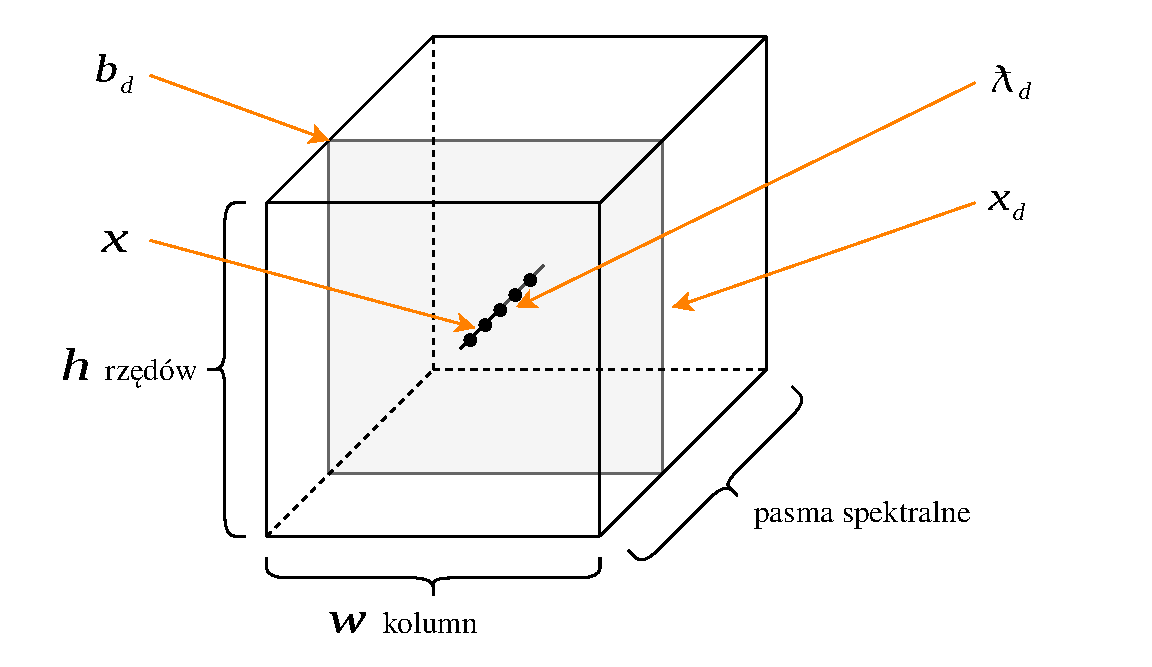
\includegraphics[width=0.75\linewidth]{rys02/multispectral-cube-vector}
	\caption{Schemat kostki wielospektralnego}
	\label{fig:multispectral-cube}	
\end{figure}

Na rysunku ~\ref{fig:multispectral-cube} zilustrowano układ danych w kostce wielospektralnej. Kostka taka składa się z~$n_x$ ($h$ rzędów na $w$ kolumn) pikseli $x$. Każdy piksel jest wektorem współczynników spektralnych o~długości  $n_D$, gdzie $n_D$ jest liczbą obrazów spektralnych, na które składa się dana wielospektralna. Każdy współczynnik $x_d$ jest wartością reakcji sensorycznej dla odpowiadającego pasma spektralnego $b_d$ skoncentrowanego wokół fali $\lambda_d$. W skrócie obraz wielospektralny jest zbiorem obrazów rejestrowanych przy użyciu fal elektromagnetycznych o~zadanych długościach. 


\subsection{Konsekwencje formatu danych}
Ze względu na swoją charakterystykę serie obrazów wielospektralnych mogą bezproblemowo osiągać rozmiary setek megabajtów, lub nawet gigabajtów. Zazwyczaj jednak obrazy są rejestrowane aparatem o~matrycy ok. 2 Mpix. Większość danych pochodnych, które są efektem analizy tego obrazu posiadają podobne rozmiary. Informacja ta jest kluczowa podczas projektowania mechanizmu zarządzania danymi w~takim systemie. Biorąc pod uwagę rozmiar danych mechanizm taki powinien:
\begin{itemize}
\item unikać tworzenia zbędnych kopi danych,
\item dokonywać obliczeń danych wyłącznie na żądanie,
\item zwalniać z~pamięci dane, które nie są już wykorzystywane przez aplikację.
\end{itemize}

\section{Dane w systemie Gerbil}

Oryginalny obraz wielospektralny jest traktowany jako dana wejściowa w systemie. Na jego podstawie powstają dane pochodne. Są to głównie kolejne obrazy oraz histogramy wielospektralne. Do stworzenia prototypu mechanizmu zarządzania danymi oraz procesem przetworzenia użyte zostały poniższe dane:
\begin{itemize}
	\item \index{image} \textbf{image} -- oryginalny obraz wielospektralny. Dana ta jest obliczana podczas inicjalizacji aplikacji. Użytkownik może wejść w interakcję z~systemem dopiero gdy image zostanie przetworzone.
	\item \index{ROI} \textbf{ROI (Region of Interest)} -- wyselekcjonowany podzbiór danych, w tym przypadku wybrane prostokątne zaznaczenie obrazu. Jest przechowywany jako współrzędne lewego górnego wierzchołka zaznaczenia, jego wysokość oraz szerokość,
	\item \index{image.IMG} \textbf{image.IMG} -- fragment obrazu oryginalnego zdeterminowany przez ROI,
	\item \index{image.NORM} \textbf{image.NORM} -- image.IMG po normalizacji wektorów składających się z~pikseli o~jednakowych współrzędnych na przestrzeni pasm spektralnych,
	\item \index{image.GRAD} \textbf{image.GRAD} -- gradient obrazu image.IMG,
	\item \index{image.PCA} \textbf{image.PCA} -- image.IMG po zastosowaniu metody PCA (analizy głównych składowych),
	\item \index{image.GRADPCA} \textbf{image.GRADPCA} -- image.GRAD po zastosowaniu metody PCA (ang. Principal Component Analysis - Analiza głównych składowych)\cite{PCA},
	\item \index{band} \textbf{bands.*.N} -- pojedynczy N-ty obraz spektralny danej reprezentacji image.* (przykładowo bands.NORM.6),
	\item \index{dist.IMG} \textbf{dist.IMG} - histogram wielospektralny obrazu image.IMG,
	\item \index{dist.tmp.IMG} \textbf{dist.tmp.IMG} - dana pomocnicza używana do uzyskania danej dist.IMG. 
\end{itemize}
Z racji, że jedne dane produkują inne, łatwo jest zdefiniować hierarchię danych w tym systemie.

\begin{figure}[ht]
	\centering
		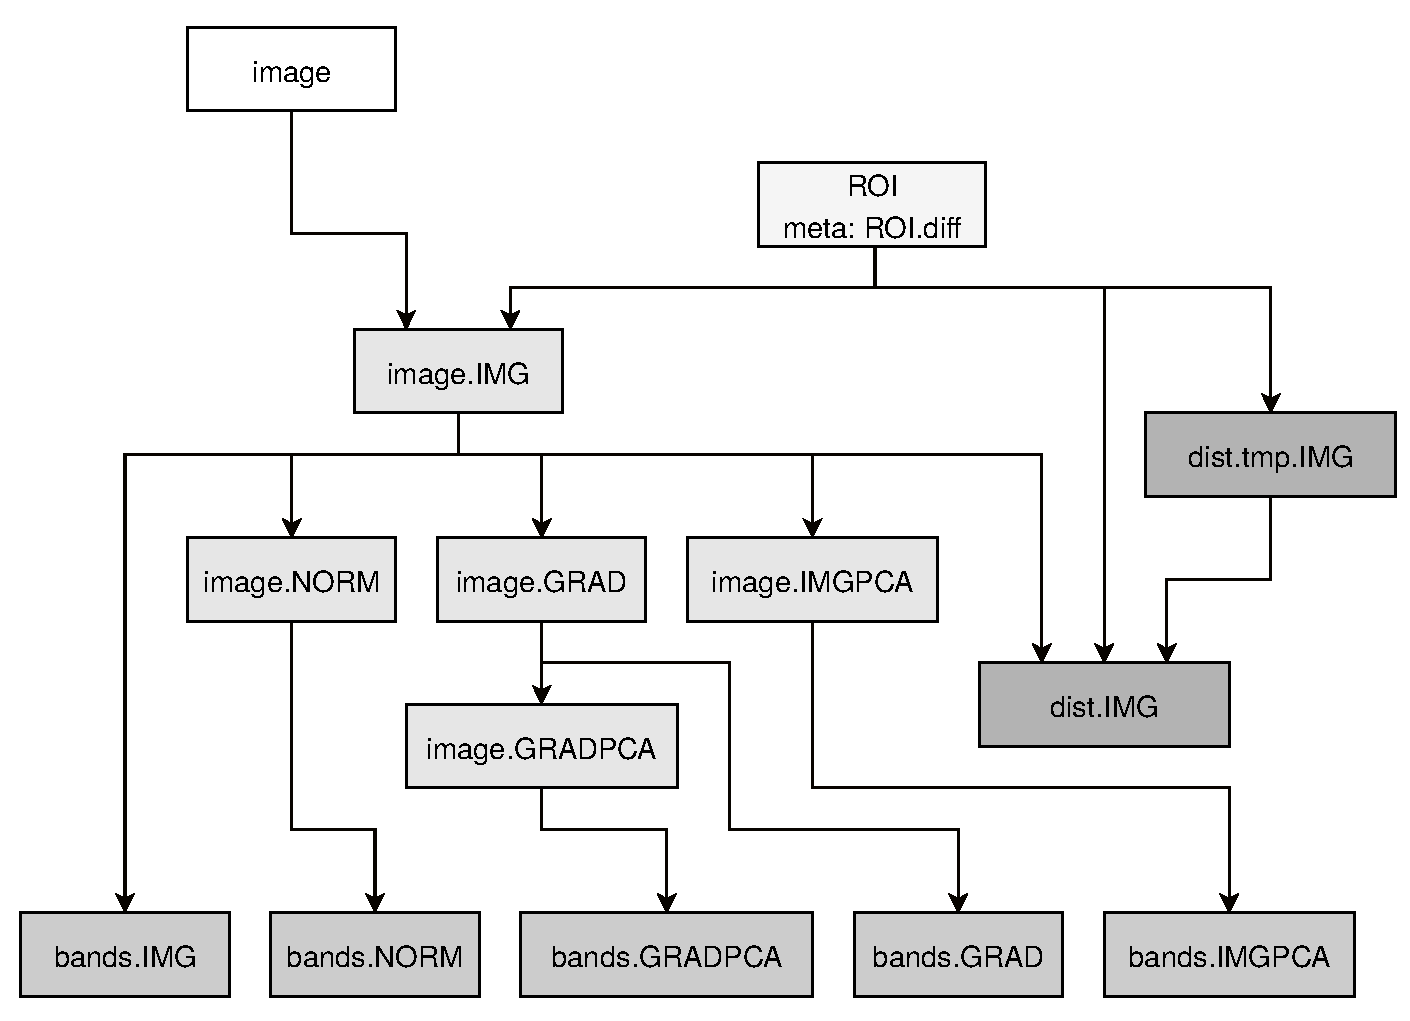
\includegraphics[width=0.7\linewidth]{rys02/data-dependencies}
	\caption{Graf zależności danych w systemie Gerbil}
	\label{fig:data-dependencies}	
\end{figure}

%\todo{Groty strzałek prawdopodobnie powinny być skierowane przeciwnie}
%\todo{Pojawiają się dziwne problemy z wstawieniem tego obrazka}

Na rysunku ~\ref{fig:data-dependencies} przedstawiono diagram zależności danych. Dane jednego koloru są do siebie semantycznie zbliżone. Przykładowo, image.NORM, image.GRAD, image.GRADPCA itp. są reprezentacjami obrazu oryginalnego. Dane posiadają również swoje metadane. Przykładowo metadaną ROI jest ROI.diff, które określa różnicę pomiędzy aktualnym a~poprzednim ROI. 

\subsection{Wpływ hierarchii danych na proces wykonania}
Analizując rysunek ~\ref{fig:data-dependencies} można dojść do wniosku, że proces przetworzenia danych jest dyktowany poprzez ich hierarchię. Przykładowo do obliczenia image.GRADPCA wymagane jest aby dane image, ROI, image.IMG oraz image.GRAD były już przetworzone. Dodatkowo można określić porządek, w którym te dane powinny zostać obliczone:

\begin{enumerate}[labelwidth=\widthof{\ref{last-item}},label=\arabic*.]
	\item image (podczas inicjalizacji systemu),
	\item ROI,
	\item image.IMG,
	\item image.GRAD,
	\item image.GRADPCA. \label{last-item}
\end{enumerate}

Scenariusz ten zakłada obliczenie każdej danej w hierarchii, co jest przypadkiem skrajnym. Często zdarza się, że pewna część danych jest aktualna. Wówczas przetwarzanie powinno rozpocząć się od pierwszej nieaktualnej danej znajdującej się najwyżej w hierarchii. 

Dodatkowo należy rozpatrzeć scenariusz równoległego wykonywania zadań. Zakładając, że aplikacja wyświetla jednocześnie dane image.NORM oraz image.GRAD, natomiast image.IMG zostało odświeżone, można dojść do wniosku, że system powinien w następnym kroku dokonać obliczeń obu danych (image.NORM i~image.GRAD). Obliczenia te można wykonać szeregowo bądź równolegle, wobec tego można zdefiniować opcjonalne wymaganie dla systemu zarządzania zadaniami jako możliwość równoległego przetwarzania zadań.

\chapter{Technologie wykorzystane w~systemie Gerbil}

Projekt jest rozwijany pod systemem operacyjnym Linux, dystrybucją Ubuntu 16.04.

\index{C++} \section{C++}
System Gerbil jest rozwijany w~języku C++. Jest to język programowania ogólnego przeznaczenia, ze szczególnym zastosowaniem w~tworzeniu systemów. C++ to język: 
\begin{itemize}
	\item wieloparadygmatowy -- pozwala na programowanie proceduralne, obiektowe, funkcyjne oraz ogólne,
	\item statycznie typowany -- zgodność typów jest sprawdzana w~trakcie kompilacji,
	\item pozwalający na bezpośrednie zarządzanie pamięcią,
	\item tworzony według zasady zerowego narzutu - elementy tego języka oraz proste abstrakcje muszą być optymalne (nie marnować bajtów pamięci ani cyklów procesora),
	\item umożliwiający tworzenie lekkich i~wydajnych abstrakcji \cite{Stroustrup}\cite{cplusplus}.
\end{itemize}

Język o~takiej charakterystyce jest dobrym wyborem do implementacji systemu analizy i~wizualizacji skomplikowanych danych.

W projekcie używany jest standard ISO/IEC 14882:2011 języka C++ oraz kompilator GCC w~wersji 5.4.0 \cite{C++11}.

\index{STL} \subsection{STL}
STL (ang. Standard Template Library) jest biblioteką standardową języka C++. Oferuje ona szereg kontenerów, klas, obiektów funkcyjnych oraz algorytmów. Składniki te opisane są w~standardzie ISO języka C++, oraz gwarantują identyczne zachowanie w~każdej implementacji \cite{Stroustrup}. Ułatwia to tworzenie aplikacji wieloplatformowych. Dzięki gotowym rozwiązaniom zawartym w~bibliotece standardowej, proces wytwarzania oprogramowania zyskuje na prostocie i~efektywności. 

\index{shared\_ptr} \subsubsection{\lstinline$shared_ptr$}
\lstinline$shared_ptr$ jest typem umożliwiającym reprezentację własności wspólnej. Wykorzystywany jest w~sytuacjach, gdy dwa (lub więcej) fragmenty kodu wymagają dostępu do danych, podczas gdy żaden nie jest odpowiedzialny za usunięcie tych danych. Obiekt \lstinline$shared_ptr$ jest rodzajem wskaźnika z~licznikiem wystąpień. Jeśli liczba obiektów wskazujących na konkretną daną spadnie do zera, dana ta jest usuwana \cite{Stroustrup}. 

\index{mutex} \subsubsection{\lstinline$mutex$}
Muteks jest obiektem typu \lstinline$mutex$, służącym do reprezentowania wyłącznych praw dostępu do konkretnego zasobu. Wykorzystuje się go do ochrony przed wyścigami do danych oraz synchronizacji dostępu do danych współdzielonych między wątkami.

Muteks może być w~posiadaniu tylko jednego wątku na raz. Zajęcie muteksu jest równoznaczne z~nabyciem wyłącznych praw własności do niego. Operacja zajmowania muteksu jest blokująca. Zwolnienie muteksu oznacza zrzeczenie się z~prawa własności do niego. Daje to możliwość zajęcia muteksu przez inne oczekujące wątki \cite{Stroustrup}.

%\subsubsection{\lstinline$condition_variable$}

\index{Qt} \section{Qt}

Qt jest platformą programistyczną wyposażoną w narzędzia pozwalające usprawnić proces wytwarzania oprogramowania oraz interfejsów użytkownika dla aplikacji desktopowych, wbudowanych bądź mobilnych \cite{Qtdoc}.

Platforma Qt posiada szerokie spektrum funkcjonalności. Między innymi są to:
\begin{itemize}
	\item system meta-obiektów,
	\item mechanizm sygnałów i~slotów służący do komunikacji pomiędzy obiektami,
	\item wbudowany system przynależności obiektów,
	\item wieloplatformowe wsparcie modułu wielowątkowości.
		
\end{itemize}

W systemie Gerbil jest wykorzystywane Qt w~wersji 5.7.

\index{sygnał} \index{slot} \subsection{Sygnały i~sloty}

Spośród rozszerzeń języka C++, jakie oferuje Qt, na szczególną uwagę zasługuje mechanizm sygnałów i~slotów. Dzięki niemu możliwe jest skomunikowanie dwóch dowolnych obiektów w~sposób alternatywny do użycia wywołań zwrotnych. 

Sygnał jest wysyłany, gdy nastąpi jakieś zdarzenie (np. naciśnięcie przycisku przez użytkownika), natomiast slot jest odpowiedzią na ten sygnał. Sygnatury sygnału i~slotu muszą być zgodne. Mechanizm ten jest luźno powiązany (ang. loosely coupled). Oznacza to, że klasa emitująca sygnał nie musi być świadoma klasy odbierającej. Sygnały i~sloty pozwalają na przekazanie dowolnej liczby argumentów dowolnego typu. Sygnały muszą zostać zadeklarowane po słowie kluczowym \lstinline$signals$. Z jednym slotem można połączyć dowolną ilość sygnałów, i~odwrotnie -- z~jednym sygnałem można skojarzyć dowolną ilość slotów.

Wszystkie klasy korzystające z~tego mechanizmu muszą w~swojej deklaracji zawierać makro \lstinline$Q_OBJECT$ oraz dziedziczyć (bezpośrednio bądź pośrednio) po klasie \lstinline$QObject$ \cite{Qtdoc}.


\subsubsection{Składnia} 
Sposób tworzenia połączeń zostanie zilustrowany na przykładzie. Za punkt wyjścia posłużą dwie klasy: \lstinline$Sender$ (Listing \ref{sender}) oraz \lstinline$Receiver$ (Listing \ref{receiver}).

\begin{minipage}{\textwidth}
	\begin{lstlisting}[label=sender,caption=Deklaracja klasy \lstinline$Sender$]
class Sender : public QObject
{
	Q_OBJECT
public:
	explicit Sender(QObject *parent = 0) : QObject(parent) {}
	
signals:
	void sendMessage(QString msg);
	
};
	\end{lstlisting}
\end{minipage}

\begin{minipage}{\textwidth}
	\begin{lstlisting}[label=receiver, caption=Deklaracja klasy \lstinline$Receiver$]
class Receiver : public QObject
{
	Q_OBJECT
public:
	explicit Receiver(QObject *parent = 0) : QObject(parent) {}
	
	void receiveMessageMethod(QString msg) {
		std::cout << "got message in method: " << msg;
	}
	
public slots:
	void receiveMessageSlot(QString msg) {
		std::cout << "got message: " << msg;
	}
};
	\end{lstlisting}
\end{minipage}

Z analizy listingów \ref{sender} oraz \ref{receiver} wynika, że klasa \lstinline{Sender} zawiera sygnał \lstinline{sendMessage}, natomiast klasa \lstinline{Receiver} zawiera publiczną metodę \lstinline{receiveMessageMethod} oraz publiczny slot \lstinline{receiveMessageSlot}.

W Qt występują dwa rodzaje składni pozwalające na ustanowienie połączenia. Jedna z~nich (starsza) pozwala na ustanowienie połączenia jedynie pomiędzy sygnałem a~sygnałem, bądź sygnałem a~slotem. Drugi rodzaj składni, wprowadzony w~Qt5, pozwala dodatkowo na nawiązanie połączenia pomiędzy sygnałem a~metodą klasy. Na listingu \ref{connectionsyntax} przedstawiony jest zarówno stary jak i~nowy zapis.

\begin{minipage}{\textwidth}
	\begin{lstlisting}[label=connectionsyntax, caption={Składnia tworzenia połączeń między obiektami},alsoletter={()[].=}]
Sender sender;
Receiver receiver;

//stara skladnia
//poprawne
QObject::connect(&sender, SIGNAL(sendMessage(QString)), &receiver, SLOT(receiveMessageSlot(QString)));
//niepoprawne
QObject::connect(&sender, SIGNAL(sendMessage(QString)), &receiver, SLOT(receiveMessageMethod(QString)));

//nowa skladnia
QObject::connect(&sender, &Sender::sendMessage, &receiver, &Receiver::receiveMessageMethod);
QObject::connect(&sender, &Sender::sendMessage, &receiver, &Receiver::receiveMessageSlot);
	\end{lstlisting}
\end{minipage}

Mechanizm sygnałów i~slotów jest powszechnie wykorzystywany w~systemie Gerbil do ustanowienia komunikacji pomiędzy obiektami. Używana jest zarówno stara jak i~nowa składnia.

\subsection{Wątek GUI oraz wątki robocze}
GUI (ang. Graphical User Interface) jest graficznym interfejsem użytkownika. Każda aplikacja jest uruchamiana w~osobnym wątku. Jest on nazywany wątkiem głównym (bądź "wątkiem GUI" w~aplikacjach Qt). Interfejs użytkownika rozwijany w~Qt musi zostać uruchomiony w~tym wątku. Wszystkie komponenty graficznego interfejsu użytkownika (ang. widget) oraz kilka klas pochodnych nie zadziałają w~wątkach pobocznych. Wątki poboczne są często nazywane "wątkami roboczymi", ponieważ wykorzystywane są aby odciążyć główny wątek od skomplikowanych obliczeń \cite{Qtdoc}. Gdyby te obliczenia były wykonywane w~ głównym wątku, aplikacja przestałaby być responsywna podczas obliczeń, co jest zawsze efektem niepożądanym.

\index{Boost} \section{Boost}
Boost jest kolekcją bibliotek do języka C++. Biblioteki te poszerzają funkcjonalności tego języka \cite{boost}. Wiele z~bibliotek rozwijanych przez Boost zostało włączonych do standardu C++. Z~perspektywy systemu Gerbil na specjalną uwagę zasługuje Boost.Any.



\subsection{Boost.Any}
W języku C++ kwestia przechowania obiektów dowolnego typu jest problematyczna, ponieważ jest to język statycznie typowany. 

\subsubsection{\lstinline$void*$}
W czystym C++ można użyć \lstinline$void*$. Do zmiennej typu \lstinline$void*$ można przypisać wskaźnik dowolnego typu poza wskaźnikiem do funkcji oraz wskaźnikiem do składowej. Aby użyć takiej zmiennej należy dokonać jawnej konwersji \lstinline$static_cast$. Do zastosowania \lstinline$void*$ w~kodzie wysokopoziomowym należy podchodzić z rezerwą. Może to wskazywać na błędy projektowe \cite{Stroustrup}.

\subsubsection{\lstinline$boost::any$}
Rozwiązaniem, które z~powodzeniem można stosować w~kodzie wysokopoziomowym jest właśnie klasa \lstinline$boost::any$. Jego zdecydowaną przewagą nad \lstinline$void*$ jest bezpieczny typowo interfejs. Jest to kontener opakowujący pojedynczy obiekt niemal dowolnego typu (obiekt musi posiadać możliwość inicjalizacji na bazie innego obiektu tego typu -- ang. copy-constructible).
Aby użyć obiektu przechowywanego przez \lstinline$boost::any$ należy dokonać rzutowania \lstinline$boost::any_cast$. Jeżeli zostanie podany typ, na który obiekt nie może zostać zrzutowany, zostanie zgłoszony wyjątek \lstinline$boost::bad_any_cast$ \cite{boost}.

\index{TBB} \section{Intel Threading Building Blocks}
Intel Threading Building Blocks (TBB) jest biblioteką szablonów ułatwiającą programowanie równoległe. W swojej ofercie posiada gotowe struktury danych oraz zrównoleglone algorytmy~\cite{tbb}.

W systemie Gerbil biblioteka TBB używana jest głownie do implementacji algorytmów przetwarzania obrazów wielospektralnych.

\index{OpenCV} \section{OpenCV}
OpenCV (Open Source Computer Vision Library) to biblioteka przeznaczona do rozpoznawania obrazów oraz uczenia maszynowego~\cite{opencv}.

Biblioteka ta znajduje wykorzystanie w~systemie Gerbil jako bogata baza struktur danych wykorzystywanych do przetwarzania obrazów oraz zaawansowanych algorytmów rozpoznawania obrazów.
\chapter{Aktualny stan projektu Gerbil}

\index{MVC} \section{Wzorzec MVC}

Aplikacja Gerbil jest zaprojektowana według wzorca MVC (Model-View-Controller) z~wykorzystaniem platformy Qt. MVC jest wzorcem architektonicznym używanym często do tworzenia interfejsów użytkownika. Podstawą MVC są trzy obiekty:
\begin{itemize}
	\item model -- komponent odpowiedzialny za serwowanie danych;
	\item widok -- komponent odpowiedzialny za wizualizację danych;
	\item kontroler -- komponent definiujący logikę, za pomocą której interfejs użytkownika odpowiada na jego żądania.
\end{itemize}
Podział tych ról można zaobserwować na rysunku ~\ref{fig:mvc}.

\begin{figure}[ht]
	\centering
	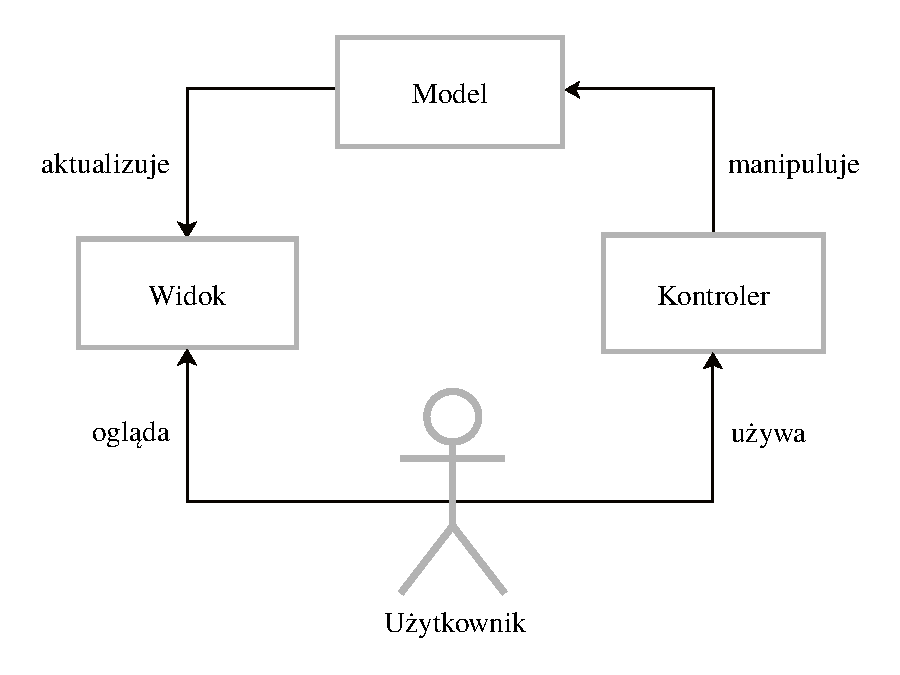
\includegraphics[width=0.7\linewidth]{rys04/mvc}
	\caption{Podział ról we wzorcu architektonicznym MVC}
	\label{fig:mvc}	
\end{figure}

Dzięki wykorzystaniu tego wzorca sposób przechowywania danych nie ma wpływu na to jak są one przedstawione użytkownikowi~\cite{Qtdoc}.

\section {Architektura aplikacji Gerbil}

W aplikacji Gerbil wzorzec MVC zastosowano w~sposób klasyczny: 
\begin{itemize}
	\item modele są odpowiedzialne za obliczenia danych oraz sygnalizowanie pojawienia się ich nowej wersji;
	\item widoki wyświetlają dane;
	\item kontrolery zajmują się kojarzeniem akcji użytkownika z~konkretną funkcjonalnością modelu.
\end{itemize}

Dodatkowo w~aplikacji występuje wątek roboczy. W nim uruchomiona jest kolejka zadań. Zadanie (obiekt klasy \lstinline$Task$) jest komponentem realizującym wykonanie czasochłonnego algorytmu analizy danych. Modele tworzą zadania i~przekazują je do kolejki. Kolejka przyjmuje zadania i~wykonuje je po kolei. W ten sposób skomplikowane obliczenia nie blokują wątku GUI, który pozostaje przez cały czas responsywny.

W takiej architekturze pojawia się problem dostępu do danych, ponieważ dwa wątki (wątek GUI, w~którym znajdują się komponenty MVC, oraz wątek roboczy, w~którym wykonywane są zadania) próbują uzyskać dostęp do tych samych danych. Zadania wykonywane w~tle powinny w~bezpieczny sposób dokonywać zapisu danych. Widoki zaś powinny być w~stanie bezawaryjnie wizualizować dane oraz dbać o~aktualność prezentowanych danych.

\subsection{Wady architektury}

System ten jest mocno zdecentralizowany. Na barkach kontrolerów spoczywa odpowiedzialność odpowiedniej propagacji sygnałów informujących o~nowej wersji danych, inwalidacji danych, jak również zapytań o~dokonanie nowych obliczeń. Prowadzi to do:
\begin{itemize}
	\item zaciemnienia kodu źródłowego zbędnymi instrukcjami warunkowymi,
	\item zignorowania pewnych sygnałów,
	\item podjęcia niewłaściwej decyzji.
\end{itemize}

Zarządzanie zadaniami również jest wadliwe. W przypadku gdy użytkownik poprzez interakcję z~systemem zleci wykonanie na raz kilku zadań dokonujących obliczeń na tych samych danych, system może zachować się w~sposób nieoczekiwany. Prowadzi to do zakończenia aplikacji z~powodu naruszenia ochrony pamięci. Nowa wersja systemu powinna w~najgorszym wypadku zakolejkować te zadania i~wykonać jedno po drugim.

Wiele komponentów interfejsu użytkownika przechowuje własne uchwyty do danych oraz ewentualnie muteks. Wobec tego same dokonują synchronizacji lub nie robią tego wcale. Nieprzemyślany model doprowadził do wielu patologii. Przykład stanowi używanie współdzielonych wskaźników do przekazywania danych, podczas gdy dane te z~założenia powinny być współdzielone.

\subsubsection{Konkluzja}

Aktualny model współdzielonych danych, w~powiązaniu z~modelem zarządzania nimi nie gwarantuje bezpiecznego dostępu do danych ani prawidłowego przebiegu procesu wykonania zadań. Biorąc pod uwagę wyżej wymienione problemy nowy mechanizm zarządzania danymi oraz procesem wykonania powinien: 
\begin{itemize}
	\item posiadać wewnętrzny mechanizm synchronizacji dostępu do danych,
	\item gwarantować bezpieczny dostęp do współdzielonych danych,
	\item gwarantować bezpieczne wykonanie zadań w~tle,
	\item gwarantować prawidłową kolejność procesu przetwarzania danych,
	\item posiadać scentralizowany mechanizm propagacji sygnałów,
	\item prawidłowo propagować informację o~dostępności nowej wersji danych,
	\item prawidłowo propagować informację o~żądaniu obliczeń nowych danych.
\end{itemize}








\bibliographystyle{plabbrv}

%UWAGA: bibliotekę referencji należy przygotować samemu. Dobrym do tego narzędziem jest JabRef.

%       Nazwę przygotowanej biblioteki wpisuje się poniżej bez rozszerzenia
%       (w tym przypadku jest to "dokumentacja.bib")

%\bibliography{dokumentacja}
%\appendix
%\include{dodatekA}
%\include{dodatekB}

\chapterstyle{noNumbered}
\phantomsection % sets an anchor
\addcontentsline{toc}{chapter}{Indeks rzeczowy}
\printindex

\end{document}
